%\documentclass{article}
%
%\usepackage{hyperref}
%\usepackage{graphicx}
%\usepackage{amsmath}
%
%\title{fa18 cs591s1: Homework 1, Problem 2}
%\author{Sarah Scheffler}
%\date{\today}

%\begin{document}
%\maketitle
\section{Problem 2}

\subsection{Problem}

In this problem, we implemented a simple algorithm to learn more than we already knew about a running counter.  
Over $n$ timesteps of data represented as an $n$-sized array of bits, $x$, running noisy counter mechanism
returned an $n$-sized array of values
\begin{align*}
    a(i) &= \sum_{j=0}^i x_j + Z_i
\end{align*}
where $Z_i$ is a uniformly randomly chosen bit.

\subsection{Algorithm}

The algorithm for with and without auxiliary information is very similar; they differ only by what we choose
for our initial guesses $\hat{x}$ are.  The algorithm is as follows:

\begin{enumerate}
    \item Inputs: 
        \begin{enumerate}
            \item $a$ = $n$-array of ``answers'' (the noisy running counter)
            \item $w$ = optional auxiliary input such that $w(i)$ has a $\frac23$ chance of matching $x(i)$.
        \end{enumerate}
    \item Set $\hat{x}$ as either
        \begin{enumerate}
            \item If we do not have auxiliary info, an $n$-sized array of random bits
            \item If we do have auxiliary guesses, set $\hat{x} = w$.
        \end{enumerate}
    \item Iterate from $i=0..n$:
        \begin{enumerate}
            \item If $a(i) = a(i-1)+2$, then we know $x(i) = 1$ because noise can only account for 1 of the
                difference between the two values.  (If $i=0$, then this condition becomes if $a(0)==2$)
            \item If $a(i) = a(i-1)-1$, then we know $x(i) = 0$. If $x(i)$ were 1, then it is impossible for
                the noisy counter to have gone \emph{down} on that $i$.
        \end{enumerate}
    \item Now we check to see if $a$ could have feasibly been generated by our $\hat{x}$, and we adjust
        $\hat{x}$ until it could have been.  We ensure that for all $i$, $\sum_{j=0}^i \hat{x}(j) + 1 \ge a(i)
        \ge \sum_{j=0}^i \hat{x}(j)$.
    \item Define the function $c(i) = \sum_{j=0}^i \hat{x}(j)$.
    \item Iterate until DONE:
        \begin{enumerate}
            \item Iterate from $i=0..n$. (inner loop)
                \begin{enumerate}
                    \item If a(i) < c(i), then set $\hat{x}(j) = 0$, where $j = argmax_{j \le i} \hat{x}(j) 
                        \ne 0$.  Then break out of inner loop.
                    \item If $a(i) > c(i)+1, then set \hat{x}(j) = 1$, where $j = argmax_{j \le i} \hat{x}(j)
                        \ne 1$.  Then break out of inner loop.
                    \item If we made it all the way to the end of the inner loop (i=n without breaking), then
                        set DONE=True.
                \end{enumerate}
        \end{enumerate}
    \item Return $\hat{x}$.
\end{enumerate}

\subsection{Results}

A graph of the results follows.  Each parameter setting was rerun 20 times.  The error bars show the standard
deviation of the results.

\begin{center}
    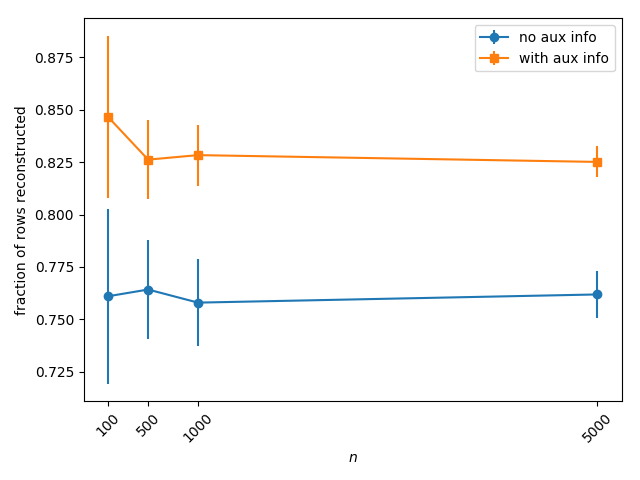
\includegraphics[width=0.5\textwidth]{running_counter.png}
\end{center}

For no auxiliary information, approximatly 76\% of the $x$ values could be
correctly guessed, regardless of $n$.  With a $2/3$ auxiliary info guess, approximately 82\% of the $x$ values
were correctly guessed.  Changing $n$ did not significantly alter the mean of the results.

A noisy counter is inapporopriate for hiding this form of information, because the differences in the
resulting queries are very easy to learn information from.  Even without auxiliary information, several
patterns of user behavior can be seen exactly (e.g. one result with noise=0 followed by a result of value=1
and noise=1 always reveals that user's value).

%\end{document}
